\chapter{State-of-the-Art}
\hspace*{6mm}
To comprehensively contemplate requirements of an endodontic robot such as workspace, payload, clinical problems, technical and clinical literatures are involved. Recent literatures have revealed that researchers have seen the use of dental robot for implant surgery \cite{Kim2009ASO}\cite{Li2019ACD}\cite{9026216}. There was a domestic team dedicating to develop an endodontic robot \cite{dong2006wip}. Endodontic file has its physical property
\section{Dental Robot}
\hspace*{6mm}There is a commercial robot, YOMI  \cite{bolding2021accuracy}. YOMI has received the clearance from FDA and has performed more than $2,700$ times surgery in the USA. In the pandemic of Covid-19 in 2020, YOMI provided non-contact surgery between dentists and patients due to its automatic robotic system. 
\begin{figure}[htbp]
\begin{center}
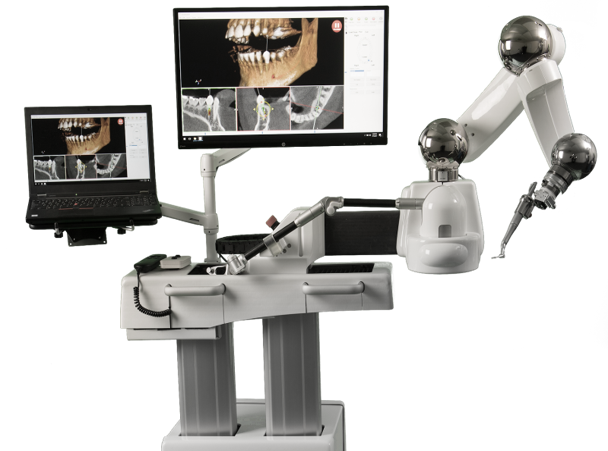
\includegraphics[width=0.9\linewidth]{Images/YOMI.png}
\caption{
YOMI
}\label{fig:YOMI}
\end{center}
\end{figure}
There is one robotic system that is designed to perform the endodontic therapy. In Intelligent Micro Robot Development for Minimum Invasive Endodontic Treatment \cite{dong2010design}, they proposed a micro robot performing root canal treatment with the assistance
of 3D computer model system. It utilizes the 3D model to plan the corresponding path to accomplish an endodontic treatment.

There are more and more robots which applied to specific surgery. In the dental field, the majority of robotic applications are in implant surgery. The researchers in Chosun University built a dental implant robot \cite{Kim2009ASO}, a remote center of motion (RCM) mechanism. Li, J. et al. designed a robotic system using a soft bracing technique to drill teeth \cite{Li2019ACD}. Also, there is the first commercial implant robot, YOMI, developed by Neosis \cite{web3}. However, there was one and only one robot for the endodontic treatment. The domestic researcher Janet Dong and his team proposed a microrobot performing root canal treatment with the assistance of a 3D computer model system. However, the study using 3D model belongs to pre-operation.
\begin{figure}[htbp]
\begin{center}
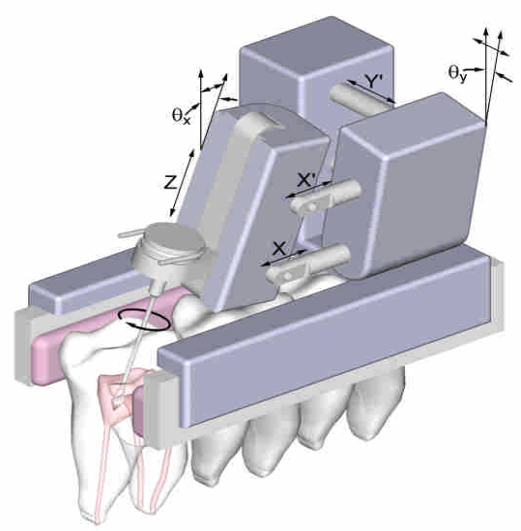
\includegraphics[width=0.7\linewidth]{Images/NCTU_1.png}
\caption{
Multi-purpose micro-machine for automatic endodontic treatment
}\label{fig:NCTU_1}
\end{center}
\end{figure}
\section{Peg-in-Hole}
\section{Torque Control}
A.	YOMI – commercial robot
B.	HK - dental implant robot
C.	Korean - dental implant robot
D.	NCTU – RCT robot

\section{File property}
\hspace*{6mm}To protect the endodontic file from fracturing, we need to be familiar with its physical property and its correct operations. We delve into the physical properties of an endodontic file. A file is made of alloys of Nickel and Titanium, which is a superelastic material. The Ni-Ti file has significantly more elastic and incorruptible properties. This feature allows it to bend when inserted into a curve root canal and thereby reduces the possibility of stuck.
\begin{figure}[htbp]
\begin{center}
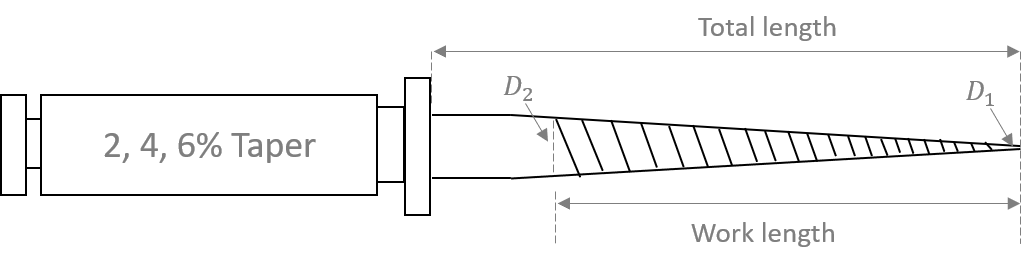
\includegraphics[width=1\linewidth]{Images/Endodontic_File.png}
\caption{The illustration of an endodontic file
}\label{fig: Endodontic File}
\end{center}
\end{figure}	
\par
In Fig \ref{fig: Endodontic File}, an endodontic file is illustrated. There are four types of total length - $21$, $25$, $28$, and $31$ mm. They all have the same work length - $16$ mm. Each file has their own number such as $\#15, \#20, \#25, \cdots, \#40$, which represent the diameter of files. Take a $\#15$ file with $2\%$ taper for example,
\par\noindent
the diameter of the tooltip $D_1$ is
\begin{equation*}
\begin{split}
15/100=0.15 \text{ (mm)}
\end{split}
\end{equation*}
and the diameter at the end of the work length $D_2$ is
\begin{equation*}
\begin{split}
0.15 + 16 \cdot 6\% = 1.11 \text{ (mm)}
\end{split}
\end{equation*}
						